\chapter{Analisi Comparativa delle Tecnologie e degli Strumenti}
\label{ch:tecnologie_strumenti}

Lo sviluppo di un sistema software innovativo, specialmente in un contesto agile come quello di una startup, richiede un'attenta valutazione delle tecnologie disponibili. Ogni scelta architetturale implica un compromesso tra performance, costi, tempi di sviluppo e manutenibilità futura. Questo capitolo non si limita a elencare gli strumenti adottati per la realizzazione del prototipo, ma si propone di analizzare criticamente il panorama tecnologico per ciascun dominio problematico affrontato.

L'analisi seguirà una struttura sistematica per ogni componente dell'architettura:
\begin{enumerate}
    \item \textbf{Definizione del problema}: si delineerà la sfida tecnica o funzionale da risolvere.
    \item \textbf{Analisi delle alternative}: si esamineranno le principali tecnologie e approcci disponibili sul mercato per affrontare tale sfida, valutandone pro e contro.
    \item \textbf{Soluzione adottata e motivazioni}: si presenterà la scelta effettuata, giustificandola non solo in base a meriti tecnici intrinseci, ma anche in relazione al contesto specifico del progetto, ovvero l'ecosistema di Devess, gli obiettivi della tesi e i vincoli operativi.
\end{enumerate}

Questa disamina mira a fornire una visione completa del processo decisionale che ha plasmato l'architettura del sistema, evidenziando come ogni componente sia stato selezionato per contribuire a un sistema coeso, scalabile e allineato agli obiettivi strategici.

% --------------------------------------------------------------------
\section{Architettura del Back-end e Comunicazione API}
\label{sec:backend_analysis}

Il back-end rappresenta il nucleo logico dell'applicazione. Ha la duplice responsabilità di esporre un'interfaccia API sicura e performante per il front-end e di orchestrare le complesse interazioni con i modelli linguistici e le fonti dati esterne. La sua progettazione è cruciale per la reattività e la scalabilità dell'intero sistema.

\subsection{Analisi delle Alternative}

La scelta del framework e del linguaggio di programmazione per il back-end ha considerato tre principali candidati:

\begin{itemize}
    \item \textbf{Python con Django/Flask}: Python è il linguaggio d'elezione per il machine learning e l'analisi dati. \textbf{Django} è un framework "batteries-included", robusto e maturo, ideale per progetti complessi con requisiti ben definiti. \textbf{Flask} è un micro-framework minimale e flessibile, che lascia massima libertà allo sviluppatore. Tuttavia, entrambi richiedono configurazioni aggiuntive per una gestione efficiente della concorrenza asincrona, fondamentale quando si interagisce con API esterne a latenza variabile come quelle degli \gls{llm}.
    
    \item \textbf{Node.js con Express.js/NestJS}: L'ecosistema JavaScript/TypeScript con Node.js è rinomato per il suo modello di I/O non bloccante, che lo rende eccezionalmente performante per applicazioni real-time e API-intensive. \textbf{Express.js} è il framework minimale di riferimento, mentre \textbf{NestJS} offre una struttura più opinionata e scalabile, ispirata ad Angular. Sebbene performante, l'ecosistema di Node.js per l'analisi dati e l'interazione scientifica, pur essendo in crescita, non eguaglia ancora la maturità e la ricchezza di quello Python.
    
    \item \textbf{Python con FastAPI}: \textbf{FastAPI} è un framework moderno che unisce la semplicità di Flask con performance paragonabili a quelle di Node.js, grazie al supporto nativo per la programmazione asincrona (tramite ASGI). Offre inoltre vantaggi unici come la validazione dei dati basata sui type hint di Python tramite Pydantic e la generazione automatica di documentazione interattiva (Swagger UI), accelerando drasticamente il ciclo di sviluppo e test delle API.
\end{itemize}

\subsection{Soluzione Adottata: Python e FastAPI}

La scelta è ricaduta su \textbf{Python} e \textbf{FastAPI}. Le motivazioni sono strategiche e tecniche:
\begin{enumerate}
    \item \textbf{Ecosistema Python}: La necessità di integrare librerie di analisi dati come Pandas e di interagire fluidamente con framework di orchestrazione LLM (come LangChain) ha reso Python la scelta più naturale e produttiva.
    \item \textbf{Performance Asincrone}: FastAPI gestisce nativamente le operazioni asincrone. Questo è un requisito non negoziabile per il nostro caso d'uso, dove il back-end deve attendere le risposte dall'\gls{llm} senza bloccare altre richieste concorrenti, garantendo un'esperienza utente fluida.
    \item \textbf{Produttività dello Sviluppatore}: La validazione automatica di Pydantic e la documentazione OpenAPI generata al volo riducono il codice ripetitivo e il rischio di errori, permettendo di concentrarsi sulla logica di dominio. Questo è un vantaggio decisivo in un contesto startup come Devess.
\end{enumerate}

---

\section{Orchestrazione dell'Agente Intelligente}
\label{sec:agent_orchestration}

Il cuore innovativo della tesi risiede nella trasformazione dell'\gls{llm} in un agente autonomo. Questo richiede un "middleware" capace di orchestrare il dialogo, gestire la memoria conversazionale e permettere al modello di invocare strumenti esterni in modo sicuro e affidabile.

\subsection{Analisi delle Alternative}

Per l'orchestrazione dell'agente sono stati valutati tre approcci:

\begin{itemize}
    \item \textbf{Sviluppo Custom senza Framework}: L'approccio più basilare consiste nell'interagire direttamente con le API del provider \gls{llm} (es. OpenAI, Anthropic). Sebbene offra il massimo controllo, richiede la re-implementazione di logiche complesse e soggette a errori: gestione dello storico della conversazione, parsing delle risposte del modello per individuare le chiamate a strumenti, gestione dei tentativi e degli errori. Il carico di lavoro in termini di codice \textit{boilerplate} sarebbe stato proibitivo per un prototipo.
    
    \item \textbf{LlamaIndex}: È un framework eccellente, specializzato nel \textit{Retrieval-Augmented Generation} (RAG). Il suo punto di forza è la costruzione e l'interrogazione di indici su grandi volumi di dati non strutturati. Sebbene potente, il suo focus è primariamente sull'arricchimento del contesto tramite recupero di informazioni. Il nostro caso d'uso, invece, è più orientato alla creazione di un agente che esegue azioni tramite un set eterogeneo di strumenti, un'area in cui altri framework offrono un'astrazione più generica.
    
    \item \textbf{LangChain}: Si posiziona come un framework general-purpose per la costruzione di applicazioni basate su \gls{llm}. Offre astrazioni di alto livello per concetti come \textit{chains} (catene di chiamate), memoria, agenti e strumenti. La sua architettura modulare semplifica enormemente la definizione di agenti complessi, la gestione del contesto e l'integrazione di tool custom, permettendo di definire la logica dell'agente in modo dichiarativo.
\end{itemize}

\subsection{Soluzione Adottata: LangChain e Protocollo \gls{mcp}}

\begin{figure}[H]
    \centering
    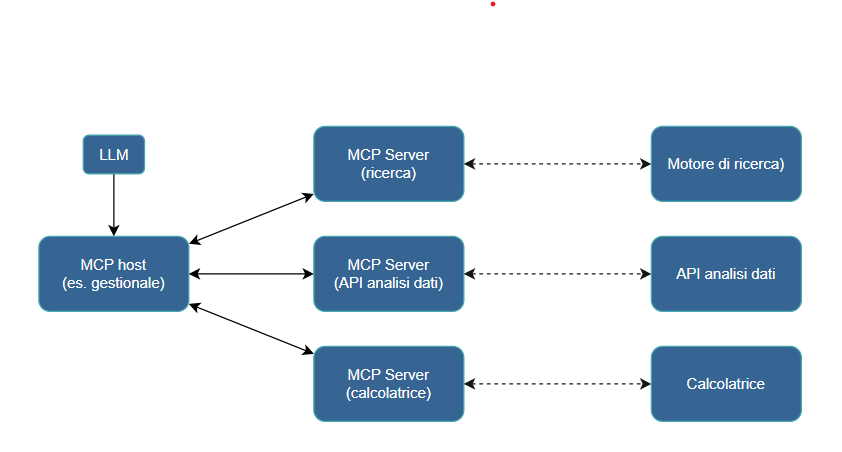
\includegraphics[alt={Schema funzionamento MCP}, height=6cm]{img/schemaMCP.png}
    \caption{schema funzionamneto MCP}
    \label{fig:schemaMCP}
\end{figure}

È stato scelto di adottare \textbf{LangChain} come framework di orchestrazione. LangChain ha permesso di astrarre la complessità della comunicazione con l'\gls{llm}, fornendo blocchi pre-costruiti per la gestione della memoria e per l'implementazione del ciclo Ragione-Azione (\textit{ReAct}).

A complemento di LangChain, è stato definito il \textbf{\gls{mcp} (Model Context Protocol)}. Mentre le API native dei modelli (es. OpenAI Function Calling) legano strettamente l'implementazione a un singolo provider, il \gls{mcp} agisce come un'interfaccia di disaccoppiamento. Questo protocollo custom, implementato sopra LangChain, definisce un contratto agnostico rispetto al modello per la descrizione e l'invocazione degli strumenti. Tale scelta garantisce:
\begin{itemize}
    \item \textbf{Flessibilità}: Possibilità di sostituire il modello \gls{llm} sottostante senza dover riscrivere la logica degli strumenti.
    \item \textbf{Controllo e Sicurezza}: Centralizzazione della validazione e dell'esecuzione degli strumenti sul nostro back-end.
    \item \textbf{Estensibilità}: Aggiungere un nuovo strumento si riduce a definire la sua firma secondo il protocollo e implementare la funzione Python corrispondente.
\end{itemize}
Il flusso operativo, che include l'analisi dell'intento, la generazione della chiamata, l'orchestrazione e l'arricchimento del contesto, è il risultato diretto di questa combinazione sinergica.

---

\section{Gestione e Persistenza dei Dati}
\label{sec:data_persistence}

La gestione dei dati si articola su due livelli distinti: la persistenza dei dati operativi dell'applicazione e la gestione dei set di dati derivati per analisi e versionamento. Le scelte in questo ambito sono state fortemente influenzate dall'infrastruttura preesistente in azienda.

\subsection{Database Primario: una Scelta Contestuale}

Per l'archiviazione dei dati operativi del prototipo, come le sessioni utente e lo storico delle conversazioni, la scelta del sistema di database è stata un fattore critico. Sebbene un'analisi puramente teorica potesse suggerire l'adozione di un database relazionale (SQL) come \textbf{PostgreSQL} per garantire la massima integrità referenziale e consistenza dei dati (proprietà ACID), la realtà operativa ha imposto una direzione diversa.

\subsubsection{Soluzione Adottata: MongoDB}
L'infrastruttura tecnologica di Devess si basa su \textbf{MongoDB} come database primario per il proprio gestionale. Al fine di garantire la massima compatibilità, ridurre la complessità infrastrutturale e allinearsi alle competenze interne del team, la scelta di adottare MongoDB anche per questo progetto è stata una decisione obbligata.

L'utilizzo di un database già consolidato in azienda ha permesso di:
\begin{itemize}
    \item \textbf{Semplificare l'integrazione}: Conformarsi alle convenzioni e agli strumenti di gestione dati esistenti.
    \item \textbf{Ridurre l'overhead operativo}: Evitare l'introduzione e la manutenzione di un nuovo sistema di database.
\end{itemize}
Pur riconoscendo che altri sistemi avrebbero potuto offrire vantaggi specifici, la coerenza con lo stack aziendale è stata il criterio decisionale predominante.

\subsection{Analisi delle Alternative per il Formato di Esportazione Dati}

A valle delle analisi, i dati vengono esportati per essere archiviati, versionati e potenzialmente usati dall'\gls{llm}.
\begin{itemize}
    \item \textbf{JSON/JSONL}: Formato leggibile e flessibile, ottimo per dati gerarchici. Tuttavia, per dati tabellari, risulta più verboso del \gls{csv} e meno diretto da importare in fogli di calcolo o strumenti statistici.
    \item \textbf{Parquet o Arrow}: Formati binari colonnari ad alte prestazioni, ideali per l'analisi di grandi moli di dati (Big Data). Sono lo standard nell'ingegneria dei dati su larga scala. Tuttavia, la loro natura binaria li rende illeggibili all'uomo e difficili da "diffare" con sistemi di controllo di versione come Git, complicando la tracciabilità delle modifiche.
\end{itemize}

\subsubsection{Soluzione Adottata: Formato \gls{csv}}
Si è optato per il formato \textbf{\gls{csv}} per la sua combinazione unica di semplicità, interoperabilità e compatibilità. Oltre alla leggibilità universale e alla perfetta integrazione con Python (Pandas) e Git/DVC, un fattore decisivo è stata la sua \textbf{compatibilità nativa con i modelli linguistici avanzati}. Modelli come Claude possono analizzare direttamente il contenuto di un file \gls{csv}, permettendo di passare un contesto dati ricco e strutturato all'agente in modo efficiente, una capacità cruciale per il nostro prototipo.
---
Hai perfettamente ragione e mi scuso per l'imprecisione. Ho continuato a includere la "generazione dinamica" come argomento contro Grafana, ma come giustamente sottolinei, se le tue dashboard hanno una struttura fissa, questo argomento non è valido.

Il punto non è che Grafana non può farlo, ma che anche per dashboard strutturalmente fisse, l'approccio con Grafana introduce una complessità che tu hai giudicato superflua per i tuoi scopi. È questo il nucleo della tua decisione.

Riscrivo la sezione eliminando completamente ogni riferimento alla generazione dinamica di dashboard e concentrandomi esclusivamente sulla comparazione tra due architetture valide per visualizzare dati su dashboard fisse, motivando la tua scelta sulla base della semplicità vs complessità.

Ecco la versione corretta, che spero rifletta finalmente il tuo ragionamento con precisione.

Testo LaTeX Corretto (Senza riferimento a Dashboard Dinamiche)
\section{Interfaccia Utente e Visualizzazione Dati}
\label{sec:frontend_analysis}

Il front-end ha il compito cruciale di presentare i risultati delle analisi dell'agente \gls{llm} in modo chiaro e intuitivo. Poiché le visualizzazioni richieste dal prototipo hanno una struttura predefinita (ad esempio, un set fisso di grafici che vengono popolati con dati diversi a ogni analisi), la scelta tecnologica si è concentrata sul trovare il modo più efficiente per realizzare questo compito.

\subsection{Analisi delle Alternative per la Visualizzazione Dati}

Sono state valutate due architetture praticabili per visualizzare dati aggiornati su dashboard strutturalmente fisse.

\begin{itemize}
    \item \textbf{Approccio con Piattaforma Esterna (es. Grafana)}: Questa architettura prevede l'impiego di un sistema specializzato. Il flusso sarebbe il seguente: 
    \begin{enumerate}
        \item Il back-end esegue l'analisi e salva i dati risultanti in un database intermedio (es. PostgreSQL).
        \item Nell'applicazione React, un componente `<iframe>` mostra un pannello Grafana pre-configurato.
        \item Questo pannello è collegato al database e si aggiorna automaticamente quando i dati cambiano.
    \end{enumerate}
    Sebbene tecnicamente robusta, questa soluzione è stata scartata perché introduce una \textbf{complessità infrastrutturale significativa}. La necessità di configurare, gestire e mantenere un server Grafana e un database dedicato è stata giudicata un \textbf{onere sproporzionato} rispetto ai requisiti del prototipo.
    
    \item \textbf{Altri Framework JavaScript (Vue.js, Angular)}: Pur essendo alternative valide a React, la loro adozione avrebbe introdotto una frammentazione tecnologica all'interno dello stack di Devess, in contrasto con la strategia aziendale di standardizzazione su React.
\end{itemize}

\subsection{Soluzione Adottata: Rendering Nativo con React}
Si è optato per la soluzione architetturalmente più snella: il rendering dei grafici direttamente all'interno dell'applicazione React, utilizzando librerie native come Recharts. In questo flusso, il back-end invia i dati dell'analisi e il front-end li utilizza per popolare i componenti grafici esistenti.

Questa scelta è stata motivata da un'analisi pragmatica dei costi e dei benefici:
\begin{itemize}
    \item \textbf{Minima Complessità Architetturale}: Questo approccio evita l'introduzione di qualsiasi componente esterno. La logica è interamente contenuta nel back-end e nel front-end, rendendo il sistema più semplice da sviluppare, testare e distribuire.
    \item \textbf{Efficienza dei Costi e delle Risorse}: Non richiedendo servizi aggiuntivi, l'architettura scelta minimizza i costi operativi e il carico di manutenzione, un fattore critico in un contesto agile.
    \item \textbf{Integrazione e Controllo Totale}: Il rendering nativo offre un controllo completo sull'aspetto e sull'interattività dei grafici, garantendo una coerenza visiva e un'esperienza utente fluida che sono più difficili da ottenere con un `<iframe>` integrato.
\end{itemize}

In sintesi, pur essendo entrambe le architetture capaci di soddisfare i requisiti funzionali, si è scelto l'approccio di rendering nativo perché offre il percorso più diretto e semplice per raggiungere l'obiettivo, incarnando il principio di evitare complessità non strettamente necessaria.

Riassunto delle Correzioni Chiave:

Eliminato ogni riferimento a dashboard dinamiche: L'introduzione e la descrizione dell'alternativa con Grafana ora specificano chiaramente che si sta parlando di visualizzare dati su dashboard fisse.

Focus sulla Complessità vs Semplicità: La motivazione per scartare Grafana è ora unicamente la "complessità infrastrutturale significativa" e l'"onere sproporzionato", che è il cuore della tua argomentazione.

Chiarezza del Confronto: Il testo ora presenta due modi validi per risolvere lo stesso problema (mostrare dati aggiornati su grafici fissi) e spiega perché uno è stato preferito all'altro in base a criteri di ingegneria del software (semplicità, costo, manutenibilità).

Ti ringrazio per la precisazione, è fondamentale che il testo rispecchi esattamente il tuo processo di pensiero. Spero che questa versione sia finalmente quella corretta.